\section{System Architecture}


\subsection{Event Schema}

All customer interactions are captured as events:

\begin{definition}[Commerce Event]
An event $e$ is a tuple $(t, c, a, p, \mathbf{x})$ where:
\begin{itemize}
    \item $t \in \mathbb{R}^+$: timestamp
    \item $c \in \mathcal{C}$: customer identifier
    \item $a \in \mathcal{A}$: action type
    \item $p \in \mathcal{P} \cup \{\bot\}$: product identifier (if applicable)
    \item $\mathbf{x} \in \mathbb{R}^k$: action-specific attributes
\end{itemize}
\end{definition}

Action types include:

\[
\mathcal{A} = \{VIEW, SEARCH, ADD\_CART, REMOVE\_CART, CHECKOUT, PURCHASE, RETURN\}
\]

\subsection{Event Processing Pipeline}

\begin{figure}[h]
\centering
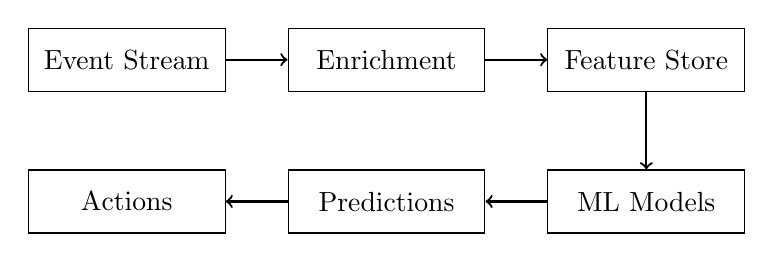
\begin{tikzpicture}[
    node distance=1.8cm,
    box/.style={rectangle, draw, minimum width=2.5cm, minimum height=0.8cm},
    arrow/.style={->, thick}
]
    \node[box] (events) {Event Stream};
    \node[box, right of=events, xshift=1.5cm] (enrich) {Enrichment};
    \node[box, right of=enrich, xshift=1.5cm] (features) {Feature Store};
    \node[box, below of=features] (models) {ML Models};
    \node[box, left of=models, xshift=-1.5cm] (predictions) {Predictions};
    \node[box, left of=predictions, xshift=-1.5cm] (actions) {Actions};

    \draw[arrow] (events) -- (enrich);
    \draw[arrow] (enrich) -- (features);
    \draw[arrow] (features) -- (models);
    \draw[arrow] (models) -- (predictions);
    \draw[arrow] (predictions) -- (actions);
\end{tikzpicture}
\caption{Analytics pipeline architecture}
\end{figure}

Events flow through:

\begin{enumerate}
    \item \textbf{Ingestion}: Kafka topics partitioned by customer ID
    \item \textbf{Enrichment}: Session attribution, product metadata, geographic data
    \item \textbf{Feature Store}: Real-time feature computation and storage
    \item \textbf{Model Serving}: Low-latency prediction endpoints
\end{enumerate}

